\documentclass[a4paper,11pt]{article}
\usepackage[T1]{fontenc}
\usepackage[a4paper,left=18mm,right=18mm,top=18mm,bottom=17mm,headheight=13pt,headsep=7mm,footskip=10mm]{geometry}
\usepackage{amsmath,booktabs,array,graphicx,tikz,xurl,listings,fancyhdr}
\usetikzlibrary{arrows.meta,positioning,calc}
\usepackage[hidelinks]{hyperref}
\renewcommand{\rmdefault}{ptm}
\renewcommand{\sfdefault}{phv}
\definecolor{Ink}{HTML}{1F2D38}
\definecolor{Blue}{HTML}{185B80}
\definecolor{Orange}{HTML}{B45E22}
\definecolor{Muted}{HTML}{536573}
\definecolor{Pale}{HTML}{EDF3F6}
\definecolor{Line}{HTML}{DCE4E9}
\definecolor{Home}{HTML}{185B80}
\definecolor{Away}{HTML}{B45E22}
% Registered submission identity. No affiliations or emails were supplied.
\newcommand{\TeamName}{Borrow Khan}
\newcommand{\TeamAuthors}{%
  Taufiq Ramadhan Ahmad, Timotius Vivaldi Gunawan, Muhammad Kevinza Faiz\\
  Viktor Arsindiantoro Siringoringo, Muhammad Neo Cicero Koda}
\newcommand{\PDFAuthors}{Taufiq Ramadhan Ahmad; Timotius Vivaldi Gunawan;
  Muhammad Kevinza Faiz; Viktor Arsindiantoro Siringoringo; Muhammad Neo Cicero Koda}
\newcommand{\CodeRevision}{8d92c6d}
\newcommand{\RepoURL}{https://github.com/taufiqrmadhana/barcahackathon}

% Generated by build.py from the committed macro-v11 report.
\newcommand{\MacroScore}{0.963966}
\newcommand{\SpellScore}{0.903226}
\newcommand{\CSVHashFirst}{6bfa4efe8c89ea9dc0030fee8ab13f8d}
\newcommand{\CSVHashLast}{8f77024b1b92024d8ee64302b1334064}

\hypersetup{pdftitle={Recovering Football Possession Spells with Tracking, Video and Temporal Consensus},
  pdfauthor={\PDFAuthors},pdfsubject={Borrow Khan -- visual technical document, Phase 1}}
\pagestyle{fancy}\fancyhf{}
\fancyhead[L]{\sffamily\scriptsize\color{Muted}BORROW KHAN\quad /\quad MORE THAN A HACK 2027}
\fancyhead[R]{\sffamily\scriptsize\color{Muted}PHASE 1}
\fancyfoot[L]{\sffamily\scriptsize\color{Muted}Code checkpoint \CodeRevision}
\fancyfoot[R]{\sffamily\scriptsize\color{Muted}\thepage\ / 4}
\renewcommand{\headrulewidth}{.3pt}
\setlength{\parindent}{0pt}\setlength{\parskip}{5pt}
\renewcommand{\baselinestretch}{1.08}
\setlength{\tabcolsep}{6pt}
\color{Ink}
\newcommand{\file}[1]{\path{#1}}
\newcommand{\heading}[1]{\par\vspace{5pt}{\sffamily\bfseries\color{Blue}\large #1}\par\vspace{2pt}}
\newcommand{\pageheading}[3]{%
  {\sffamily\scriptsize\bfseries\color{Blue}#1\quad /\quad BORROW KHAN TECHNICAL DOCUMENT}\par
  \vspace{3pt}{\sffamily\bfseries\fontsize{22}{25}\selectfont #2}\par
  {\color{Muted}#3}\par\vspace{6pt}}
\newcommand{\metric}[3]{\colorbox{Pale}{\begin{minipage}[c][17mm][c]{.22\linewidth}
  \centering{\sffamily\bfseries\fontsize{20}{23}\selectfont\color{Blue}#1}\par
  {\sffamily\small\bfseries #2}\par{\scriptsize\color{Muted}#3}\end{minipage}}}
\newcommand{\captionline}[1]{\par{\small\raggedright\color{Muted}#1\par}}
\newcommand{\notice}[1]{\par\colorbox{Pale}{\parbox{\dimexpr\linewidth-2\fboxsep\relax}{\small #1}}\par}
\lstset{basicstyle=\ttfamily\footnotesize,breaklines=true,columns=fullflexible,
  keepspaces=true,showstringspaces=false,frame=single,rulecolor=\color{Line},
  backgroundcolor=\color{Pale},framerule=.3pt,aboveskip=4pt,belowskip=4pt,
  xleftmargin=3pt,xrightmargin=3pt}
\begin{document}

{\sffamily\scriptsize\bfseries\color{Blue}SHORT TECHNICAL DOCUMENT\quad /\quad TEAM \MakeUppercase{\TeamName}}\par
\vspace{4pt}
{\sffamily\bfseries\fontsize{23}{27}\selectfont Recovering football possession spells}\par
{\sffamily\fontsize{16}{21}\selectfont with tracking, video and temporal consensus}\par
\vspace{5pt}
{\small\TeamAuthors}\par
\vspace{7pt}
\metric{0.875}{Spell-F1}{Public OOF evaluation}\hfill
\metric{0.95613}{Macro-F1}{Home / away / dead}\hfill
\metric{14 / 17}{GT spells matched}{15 predicted spells}\hfill
\metric{5 folds}{Time-based validation}{5-second purge}
\vspace{5pt}

We reconstruct possession from noisy tracking and tactical video. A physical
 decoder preserves continuity; complementary video predictions then repair short
team oscillations and possession boundaries. The output is one H/A/D/X label
for each of 199,319 tactical frames at 25\,Hz~\cite{challenge}.

\heading{1\quad System at a glance}
\begin{center}
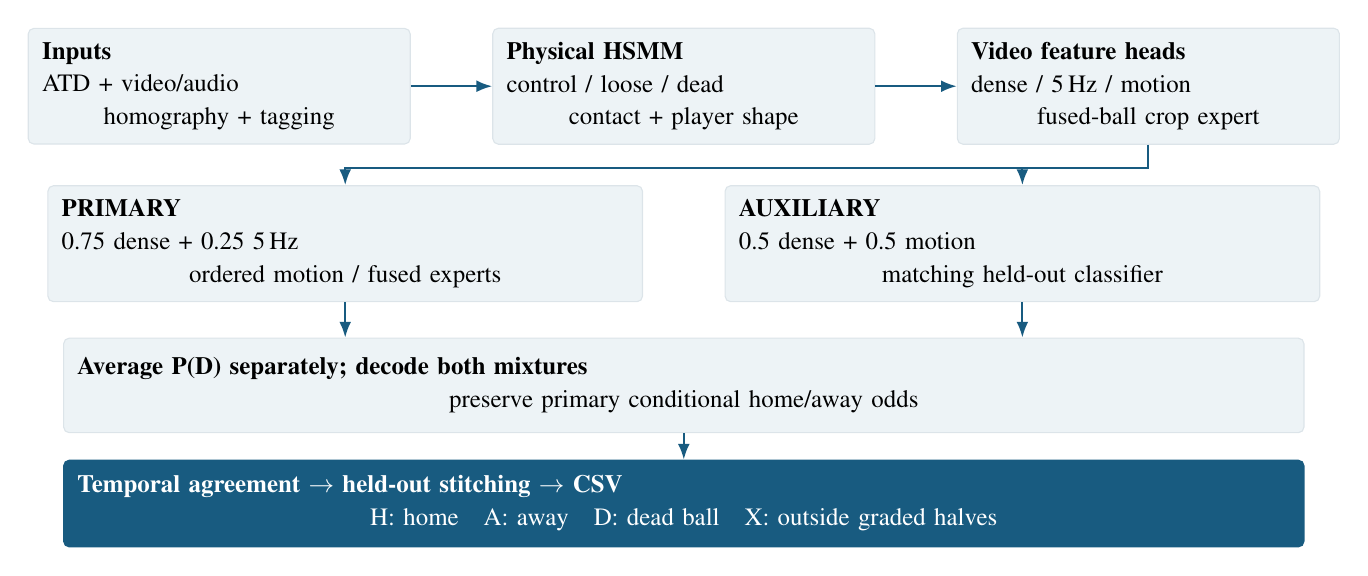
\begin{tikzpicture}[font=\small,
 box/.style={draw=Line,rounded corners=2pt,align=center,inner sep=5pt,
             minimum height=13mm,text width=45mm,fill=Pale},
 wide/.style={box,text width=72mm},
 link/.style={-{Latex[length=2mm]},draw=Blue,thick}]
\node[box] (input) at (2.6,0) {\textbf{Inputs}\newline ATD + video/audio\newline homography + tagging};
\node[box] (physical) at (8.5,0) {\textbf{Physical HSMM}\newline control / loose / dead\newline contact + player shape};
\node[box] (heads) at (14.4,0) {\textbf{Video feature heads}\newline dense / 5\,Hz / motion\newline fused-ball crop expert};
\node[wide] (primary) at (4.2,-2.0) {\textbf{PRIMARY}\newline 0.75 dense + 0.25 5\,Hz\newline ordered motion / fused experts};
\node[wide] (aux) at (12.8,-2.0) {\textbf{AUXILIARY}\newline 0.5 dense + 0.5 motion\newline matching held-out classifier};
\node[box,text width=154mm,minimum height=12mm] (decode) at (8.5,-3.8)
 {\textbf{Average P(D) separately; decode both mixtures}\newline preserve primary conditional home/away odds};
\node[box,text width=154mm,minimum height=11mm,fill=Blue,text=white,draw=Blue] (output) at (8.5,-5.3)
 {\textbf{Temporal agreement $\rightarrow$ held-out stitching $\rightarrow$ CSV}\newline
 H: home\quad A: away\quad D: dead ball\quad X: outside graded halves};
\draw[link] (input)--(physical);\draw[link] (physical)--(heads);
\draw[link] (heads.south)--++(0,-.3)-|(primary.north);
\draw[link] (heads.south)--++(0,-.3)-|(aux.north);
\draw[link] (primary.south)--(primary.south|-decode.north);
\draw[link] (aux.south)--(aux.south|-decode.north);
\draw[link] (decode)--(output);
\end{tikzpicture}
\end{center}
\captionline{Figure 1. Physical context supports both video mixtures. All temporal operations
run inside each matching held-out head, before the public slices are joined.}

\heading{Assets and their roles}
{\small\renewcommand{\arraystretch}{1.13}
\begin{tabular}{@{}p{.27\linewidth}p{.69\linewidth}@{}}
\toprule
\textbf{Asset} & \textbf{Use in the submitted system}\\\midrule
ATD + homography & Clean/fuse ball positions; measure player motion, control and contact.\\
Tactical video/audio & YOLO11s ball candidates~\cite{yolo}; frozen FILM residuals~\cite{film}; whistle and scoreboard cues.\\
Tagging + metadata & Teams, set pieces, restarts and official kick-off timing.\\
Metrica games 1--3 & Event-derived weak labels train external ownership, transition and player-shape models~\cite{metrica}.\\
\bottomrule
\end{tabular}}
\captionline{Broadcast video is unused. The physical decoder's broad phase-team prior has
zero direct weight; legacy video context retains its own configured features.}
{\small\textbf{Model provenance.} YOLO11s is COCO-pretrained and exported to OpenVINO
(INT8 calibration: 200 unlabelled crops). Frozen FILM uses $t\pm2$ frames and
$256\times192$ crops. External histogram-boosting models use clean/corrupted Metrica
tracking and weak event labels. Base shape self-training uses 8 time blocks, a 10\,s
guard and 2 rounds; external shape replaces its conditional H/A ratio only.}

\newpage
\pageheading{02}{How predictions become possessions}{Two conservative temporal rules repair short disagreements.}

\heading{1\quad Remove short ownership oscillations}
\begin{minipage}[c]{.57\linewidth}
\centering
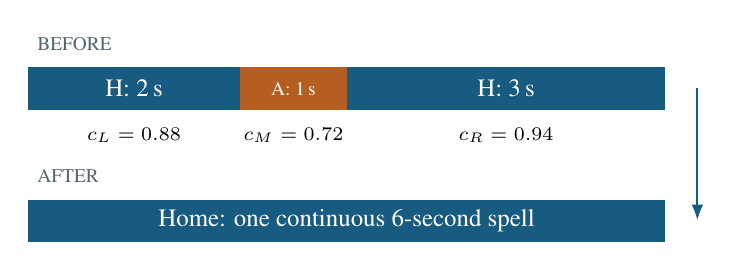
\begin{tikzpicture}[font=\small,x=1.35cm,y=1.2cm]
\node[anchor=west,font=\scriptsize\color{Muted}] at (0,1.15) {BEFORE};
\fill[Home] (0,.45) rectangle (2,.9);
\fill[Away] (2,.45) rectangle (3,.9);
\fill[Home] (3,.45) rectangle (6,.9);
\node[text=white] at (1,.675) {H: 2\,s};
\node[text=white,font=\scriptsize] at (2.5,.675) {A: 1\,s};
\node[text=white] at (4.5,.675) {H: 3\,s};
\node[font=\scriptsize] at (1,.18) {$c_L=0.88$};
\node[font=\scriptsize] at (2.5,.18) {$c_M=0.72$};
\node[font=\scriptsize] at (4.5,.18) {$c_R=0.94$};
\node[anchor=west,font=\scriptsize\color{Muted}] at (0,-.25) {AFTER};
\fill[Home] (0,-.95) rectangle (6,-.5);
\node[text=white] at (3,-.725) {Home: one continuous 6-second spell};
\draw[-{Latex[length=2mm]},Blue,thick] (6.3,.68)--(6.3,-.72);
\end{tikzpicture}
\end{minipage}\hfill
\begin{minipage}[c]{.39\linewidth}
\textbf{Apply only when:}\par
Each of the three spells is at most 4\,s; both neighbours support their team
above chance; pooled neighbour confidence exceeds the middle's confidence.
\[
\frac{2(0.88)+3(0.94)}{2+3}=0.916>0.72
\]
Select disjoint proposals once. Merges do not cascade.
\end{minipage}
\captionline{Figure 2. Illustrative timeline, not measured match data. Confidence is
conditional on alive play. The rule is symmetric for H/A/H and A/H/A.}

\heading{2\quad Extend short spells that both models support}
\begin{minipage}[c]{.57\linewidth}
\centering
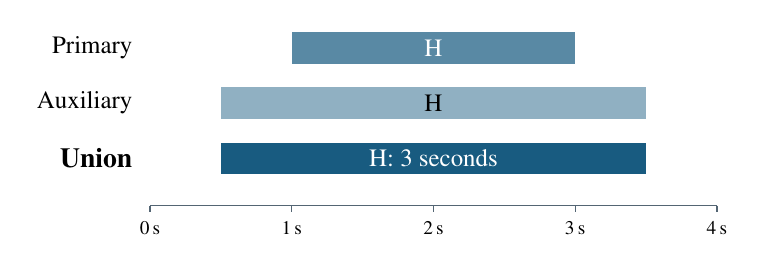
\begin{tikzpicture}[font=\small,x=1cm,y=1cm]
\node[anchor=east] at (1.5,1.0) {Primary};
\node[anchor=east] at (1.5,.3) {Auxiliary};
\node[anchor=east,font=\bfseries] at (1.5,-.4) {Union};
\fill[Home!72] (3.4,.8) rectangle (7,1.2);
\fill[Home!48] (2.5,.1) rectangle (7.9,.5);
\fill[Home] (2.5,-.6) rectangle (7.9,-.2);
\node[text=white] at (5.2,1) {H};\node at (5.2,.3) {H};
\node[text=white] at (5.2,-.4) {H: 3 seconds};
\draw[Muted] (1.6,-1)--(8.8,-1);
\foreach \i in {0,1,2,3,4}{\draw[Muted] ({1.6+1.8*\i},-1)--++(0,-.08);
 \node[font=\scriptsize,below] at ({1.6+1.8*\i},-1.08) {\i\,s};}
\end{tikzpicture}
\end{minipage}\hfill
\begin{minipage}[c]{.39\linewidth}
\textbf{Apply only when:}\par
Same team; IoU $\geq0.5$; union $\leq4$\,s; both models cover the entire union;
primary labels are all H/A.
\[
\operatorname{IoU}=\frac{2\,\mathrm{s}}{3\,\mathrm{s}}=0.667
\]
Higher-IoU proposals win conflicts. D/X and half boundaries stay fixed.
\end{minipage}
\captionline{Figure 3. Illustrative intervals: primary [1,3] s, auxiliary [0.5,3.5] s.
Only an existing, mutually supported short possession is extended.}

\heading{Physical rules and model settings}
{\small\renewcommand{\arraystretch}{1.22}
\begin{tabular}{@{}p{.24\linewidth}p{.72\linewidth}@{}}
\toprule
\textbf{Situation} & \textbf{Implemented decision}\\\midrule
Pass / loose ball & Retain the last team in its loose state; a team change requires the other control state.\\
Contact / challenge & Carry: within 1.5\,m and relative speed $\leq1.5$\,m/s. Kick: velocity-change peak $\geq2$\,m/s within 2\,m; opponent at least 0.5\,m farther.\\
Stoppage / restart & D chain: 100 frames minimum. Exit D into control. Official kick-off timing and confirmed goal-to-restart intervals provide structural D.\\
Video / half boundaries & D edges can move by at most 12 frames; preserve phase centres. No temporal edit crosses D/X, absent video or a half boundary.\\
Video heads & Logistic regression, 34 continuous/video features (+6 for motion), 301 native 1\,Hz public rows; $C=1$ dense/motion, $C=3$ 5\,Hz/fused.\\
Experts / fusion & Use expert H/A only if primary confidence $<0.8$ and expert $>0.9$. Average P(D) 50:50; retain primary H/A odds.\\
\bottomrule
\end{tabular}}
\captionline{Additional safeguards: contact vote abstains beyond 5 s from a ball observation;
existing confidence pruning removes unsupported team islands of at most 100 frames.
Feature interpolation does not bridge sampling gaps over 1 s.}

\newpage
\pageheading{03}{What improves, and how we tested it}{Public spell recovery rises while macro-F1 remains high.}

\heading{Ablation: separate the contribution of each step}
\begin{center}\includegraphics[width=\linewidth]{figures/ablation.pdf}\end{center}
\captionline{Figure 4. Same five-fold protocol and physical baseline. Bars start at zero;
annotations give exact scores. Temporal cleanup drives the spell-F1 gain.}

\notice{\textbf{Final public result:} 14 matched spells, 1 spurious prediction and 3 missed GT
spells. At every official IoU threshold (0.3--0.7), spell-F1 is
$2\times14/(15+17)=0.875$. H/A/D class F1 is 0.955923 / 0.970389 / 0.942077.}

\heading{Sensitivity to the time partition}
\begin{center}\includegraphics[width=\linewidth]{figures/fold_sensitivity.pdf}\end{center}
\captionline{Figure 5. Both mixtures are refitted at each fold count. Final macro-F1 improves
in all four checks; spell-F1 never decreases. These are repartitions of the same 17
possessions, not independent validation. Short-spell agreement alone regresses at four folds.}

\heading{Validation happens before the public slices are stitched}
\begin{center}
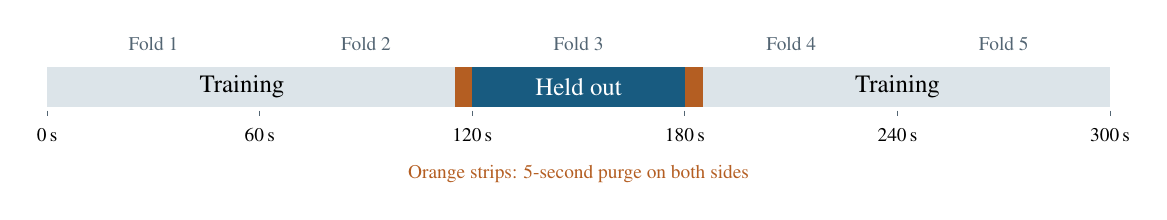
\begin{tikzpicture}[x=.045cm,y=1cm,font=\small]
\foreach \f in {1,2,3,4,5}{\node[font=\scriptsize\color{Muted}] at ({60*\f-30},.8) {Fold \f};}
\fill[Line] (0,0) rectangle (115,.5);
\fill[Orange] (115,0) rectangle (120,.5);
\fill[Blue] (120,0) rectangle (180,.5);
\fill[Orange] (180,0) rectangle (185,.5);
\fill[Line] (185,0) rectangle (300,.5);
\node at (55,.25) {Training};\node[text=white] at (150,.25) {Held out};
\node at (240,.25) {Training};
\foreach \t in {0,60,120,180,240,300}{\draw[Muted] (\t,-.05)--(\t,-.12);
 \node[font=\scriptsize,below] at (\t,-.15) {\t\,s};}
\node[font=\scriptsize\color{Orange}] at (150,-.85) {Orange strips: 5-second purge on both sides};
\end{tikzpicture}
\end{center}
\captionline{Figure 6. Example held-out fold. Primary, auxiliary and expert heads exclude the
same target labels. Each decodes the whole halves; temporal edits run before copying its slice.
All-public refits are used only outside the public window.}

\notice{\textbf{Scope of the evidence.} The public slice is 7,500 frames (5 minutes).
Feature, weight and rule selection reuses these labels. OOF fitting therefore does not remove
selection bias. Private and unseen-match performance remain unknown.}

\newpage
\pageheading{04}{Match statistics, limits and reproduction}{Predicted football summaries and a verifiable output file.}

\begin{center}\includegraphics[width=\linewidth]{figures/match_statistics.pdf}\end{center}
\captionline{Figure 7. Model predictions across 158,857 graded frames. Alive-time percentages
exclude D; spell counts include only H/A. Full-match GT is unavailable.}
\vspace{4pt}
\metric{402}{Possession spells}{204 first half / 198 second}\hfill
\metric{8.52 s}{Mean spell length}{Home 10.43 s / away 6.67 s}\hfill
\metric{46.08\%}{Dead-ball share}{Of graded time}\hfill
\metric{130}{Dead intervals}{Counted separately by half}

\heading{Limitations and next steps}
Three public spells remain missed. Occlusion and crop alignment limit contact evidence;
temporal rules can suppress real turnovers. Metrica weak labels and recording-specific
whistle/scoreboard settings limit transfer. Next: independently labelled matches,
better contact localisation and confidence calibration. The system uses offline context.
Trees, denser raw video, gap-kick and pose trials did not improve this checkpoint.

\heading{Reproduce the frozen checkpoint}
The public \file{taufiq} branch at \texttt{\CodeRevision} uses
\file{src/configs/macro_v5.json} and Python 3.11. Dependencies are pinned in
\file{requirements-src.txt}; CV/FILM use separate environments. Prepare the provided
bundle and regenerate model/video caches first: commands are in \file{src/README.md},
\file{src/bench/README.md} and \file{src/MACRO_V4.md}/\file{src/MACRO_V5.md}.
\begin{lstlisting}
OMP_NUM_THREADS=3 OPENBLAS_NUM_THREADS=3 .venv/bin/python src/run.py \
  --params src/configs/macro_v5.json --name Borrow_Khan
.venv/bin/python evaluation/validate_submission.py evaluation/results/Borrow_Khan.csv
.venv/bin/python evaluation/run_evaluation.py --gt public --bootstrap 0 --no-detail
\end{lstlisting}
{\small Expect 199,319 output rows. The scorer reads every CSV in its results directory.
All 48 contract tests passed; prototype, builder, production and tuner agree on every frame.
The full CSV checksum, metrics and asset hashes are recorded in
\file{src/bench/results/macro_v5_2026-11-16.json}.}

{\small Metrica Sports is acknowledged under its source terms; FILM uses Apache-2.0;
YOLO11 follows upstream terms. Match assets and generated model/video caches are
outside the public Git tree.}
{\footnotesize\setlength{\parskip}{0pt}
\begin{thebibliography}{4}\setlength{\itemsep}{0pt}
\bibitem{challenge} More than a Hack 2027, ``Phase 1: Ball Possession,'' 2026.
\url{https://github.com/taufiqrmadhana/barcahackathon/tree/b8e4ad0}.
\bibitem{yolo} Ultralytics, ``YOLO11.'' \url{https://docs.ultralytics.com/models/yolo11/}.
\bibitem{film} F. Reda et al., ``FILM: Frame Interpolation for Large Motion,'' ECCV, 2022.
\url{https://github.com/google-research/frame-interpolation}.
\bibitem{metrica} Metrica Sports, ``Sample tracking and event data,'' games 1--3.
\url{https://github.com/metrica-sports/sample-data}.
\end{thebibliography}}
\end{document}
